\documentclass[12 pt , a4 paper , twoside , openright ]{book}
%\part{}, \chapter{}, \section{}, \subsection{}, \subsubsection{}, \paragraph{}, \subparagraph{}
\usepackage{titlesec}
\usepackage{mathptmx}   % Carattere Times New Roman
\usepackage[a4paper, top=3cm, bottom=3cm, outer=2cm, inner=3cm]{geometry} % Impostazione dei margini
\usepackage{setspace}   % Per l'interlinea
\onehalfspacing         % Interlinea 1,5
\usepackage{hyperref}
\usepackage{graphicx}
\usepackage{datatool}
\usepackage{enumitem}

\newcommand{\sortitem}[1]{%
  \DTLnewrow{list}
  \DTLnewdbentry{list}{Description}{#1}
}

\newenvironment{sortedlist}{\DTLifdbexists{list}{\DTLcleardb{list}}{\DTLnewdb{list}}}{%
  \DTLsort{Description}{list}%
  \begin{enumerate}%
    \DTLforeach*{list}{\theDesc=Description}{%
      \item \theDesc
    }%
  \end{enumerate}%
}


\titleformat{\chapter}[hang]{\normalfont\Huge\bfseries}{\thechapter}{1em}{}

\begin{document}

\frontmatter
\begin{titlepage}
    \centering
    
\includegraphics[width=2cm]{GRAPHS/logounipd.png}

    \vspace{1cm}
    {\large UNIVERSITÀ DEGLI STUDI DI PADOVA}

    \vspace{1cm}
    {DIPARTIMENTO DI SCIENZE ECONOMICHE ED AZIENDALI "M. FANNO"}

    \vspace{0.3cm}
    {CORSO DI LAUREA MAGISTRALE IN ECONOMICS AND FINANCE}

    \vspace{3.5cm}
    {TESI DI LAUREA}

    {TITOLO}

    \vspace{4cm}
    \begin{flushleft}
        RELATORE:
        
        CH.MA PROF.SSA: ELISA TOSETTI
    \end{flushleft}

    \vspace{1cm}

    \begin{flushright}
        LAUREANDA: JESSICA CREMONESE
        
        MATRICOLA N°: 2023147
    \end{flushright}

    \centering 
    \vfill
    {ANNO ACCADEMICO 2023-2024}
\end{titlepage}

%   DICHIARAZIONE   ANTIPLAGIO
Dichiaro di aver preso visione del “Regolamento antiplagio” approvato dal Consiglio del Dipartimento di Scienze Economiche e Aziendali e, consapevole delle conseguenze derivanti da dichiarazioni mendaci, dichiaro che il presente lavoro non è già stato sottoposto, in tutto o in parte, per il conseguimento di un titolo accademico in altre Università italiane o straniere. Dichiaro inoltre che tutte le fonti utilizzate per la realizzazione del presente lavoro, inclusi i materiali digitali, sono state correttamente citate nel corpo del testo e nella sezione ‘Riferimenti bibliografici’. 

\emph{I hereby declare that I have read and understood the “Anti-plagiarism rules and regulations” approved by the Council of the Department of Economics and Management and I am aware of the consequences of making false statements. I declare that this piece of work has not been previously submitted – either fully or partially – for fulfilling the requirements of an academic degree, whether in Italy or abroad. Furthermore, I declare that the references used for this work – including the digital materials – have been appropriately cited and acknowledged in the text and in the section ‘References’. }

%   FIRMA
\vspace{2cm}
\begin{flushright}
    Firma (signature):

    
\includegraphics[width=4cm]{GRAPHS/firma_Jessica_Cremonese.jpg}
\end{flushright}


\tableofcontents


\mainmatter
    \chapter*{Introduction}

% frame the problem
% give idea of what will be done in thesis
% don't be too detailed

% DO IT LAST
    \chapter{Mental Health}

% frame the chapter
Increasingly recognized as a crucial factor for well-being, mental health carries significant economic implications that are often overlooked in favor of more easily quantified conditions, such as physical health. Nevertheless, recent events such as the COVID-19 pandemic shed light on the importance of psychological welfare. 

% economic relevance (social capital, productivity)
Mental health is an economically relevant phenomenon with far-reaching implications that extend beyond individual well-being. Poor mental health often leads to reduced productivity, increased absenteeism, and higher turnover rates in the workplace, directly impacting an organization's bottom line (OECD/EU (2018), OECD/EU (2022)). Furthermore, it places a significant burden on healthcare systems through increased medical costs and utilization of services. The indirect costs, such as loss of income due to disability and the ripple effects on families and communities, further amplify its economic relevance and far outweigh the direct healthcare costs (OECD/EU (2022), WHO (2022)). Therefore, investing in mental health not only enhances individual quality of life but also has the potential for significant economic returns, framing it as a key opportunity in the context of social capital accumulation.

This chapter aims to shed light on the definitions, statistics and dynamics of the topic, with the aim of providing the reader with comprehensive and up to date knowlege in this realm. 

\section{Defining mental health}
% what is MH in general 
    Mental health can be defined as a state of psychological well-being which allows people to cope with demands of life, realize their abilities, learn and work well while contributing to their community. It represents a crucial feature of personal and collective socio-economic develpoment, involving psychological, emotional and social welfare, and affecting how people think, feel and act. 
    Being mentally healthy goes beyond the mere absence of clinically relevant conditions, it encompasses self-esteem, resilience, relationships. Conditions that affect mental health include mental disorders, psychosocial disabilities and mental states associated with impaired functioning, or risk of self-harm. Those affected by these conditions are more likely to report lower mental well-being. 

    % MH risk factors
    Mental health is dynamic and is affected by the interplay of biological factors, environmental conditions and individual experiences. Biological factors such as genetics or substance abuse can create vulnerabilities in all stages of life, but events that occur during developmentally sensitive periods are particularly impactful. Harsh childhood experiences in the form of bullying, physical or psychological abuse and poor health can have long lasting negative consequences on an individuals' mental condition. On the other hand, mental resilience can be promoted through building social and emotional skills, providing youths with positive interactions, safety and community as well as quality education. 
    Thus, mental health can be though of as a continuum ranging from an optimal state of well being, to debilitating states of great suffering and emotional pain (WHO, 2022).

    When dealing with circumstances that can exacerbate mental ill-health, a distinction can be made between local factors which affect individuals, families and communities on a small scale, and global or systemic factors which generate vulnerabilities for the entire population. Among the latter we find key threats such as economic crises, disease outbreaks, humanitarian emergencies, displacement and climate crisis related events, as well as sociocultural and geopolitical factors such as infrastructure, inequality, social stability and environmental quality. 
    
    % MH protective factors
    Although exposure to risk factors undermines mental health, most at-risk people will not develop conditions, while many without known risk factors will develop them. In this perspective, encouraging protective factors strenghtens resilience in the population. On the individual plane, building strong social and emotional skills, a solid sense of self-worth and healthy habits such as keeping physically active are key in generating resilient individuals. Other individual protective factors include a nurturing and supportive family environment from a very young age, decent working conditions and a cohesive social network. On the structural level, protective factors manifest in economic security, easy and equal access to services, social protection, qualitable infrastructure and economic security, as well as social integration and contained inequality.  


        



\section{Global epidemiological overview}
    % define relevant MH issues --> depression, anxiety, suicide stats
    Mental health conditions are prevalent in the population, with about one in eight people worldwide living with a mental disorder (WHO, 2022). Heterogeneity in their distribution emerges according to age, gender and other individual characteristics. Overall, disorders related to anxiety and depression are the most common, and suicide accounts for more than one out of one hundred deaths (WHO, 2022). 
    % seeking help
    Still, seeking help for mental health conditions is hindered by low mental health literacy, poor service quality, high cost of care, fear of stigma and discrimination, making for underdiagnosis of all conditions. 

    % service provision not commisurated with needs
    Worldwide, mental health conditions are severely underserviced due to lack of information and research, as well as deficient provision of resources and services. On average, less than 2\% of health care budgets are dedicated to mental health, and out of that more than 70\% of mental health expenditure in middle-income countries is dedicated to psychiatric hospitals (WHO, 2022). 
    Furthermore, professionals such as psychiatrists and psychologists are scarce relative to the population, and gaps in service coverage are amplified by quality and cost of care across countries. 
    % measurement challenges
    Additionally, measurement of mental health condition is hampered by incomplete data, outdated information and cross-cultural differences in the conceptualization and tracking of conditions.

    % quick stats
    The most commonly occurring mental conditions are anxiety disorders, which have a prevalence rate of about 4\%, followed closely by depressive disorders at 3.8\%. Developmental disorders and Attention Deficit Hyperactivity Disorder (ADHD) are also significant, contributing to an additional 1.4\% and 1.1\% of cases, respectively (WHO, 2022).
    A higher percentage of the population is diagnosed in high-income countries, followed in order by middle and low-income countries (WHO, 2022). On average, people with severe mental conditions die 10-20 years prematurely with respect to the general population (Chesney et al., 2014) and at great individual and societal cost. 
    % this section
    This section presents current statistics on the global prevalence and diversity of mental health conditions, with a particular emphasis on the OECD region prior to the COVID-19 pandemic. Before delving into a data-driven discussion on this subject, it is essential to first clearly define the two most pertinent categories of mental disorders under consideration: anxiety and depressive disorders. 


        % anxiety       [  %  TO DO  %  ]
        \subsection{Anxiety disorders}

            \begin{figure}  % anxiety OECD rates figure
                \centering
                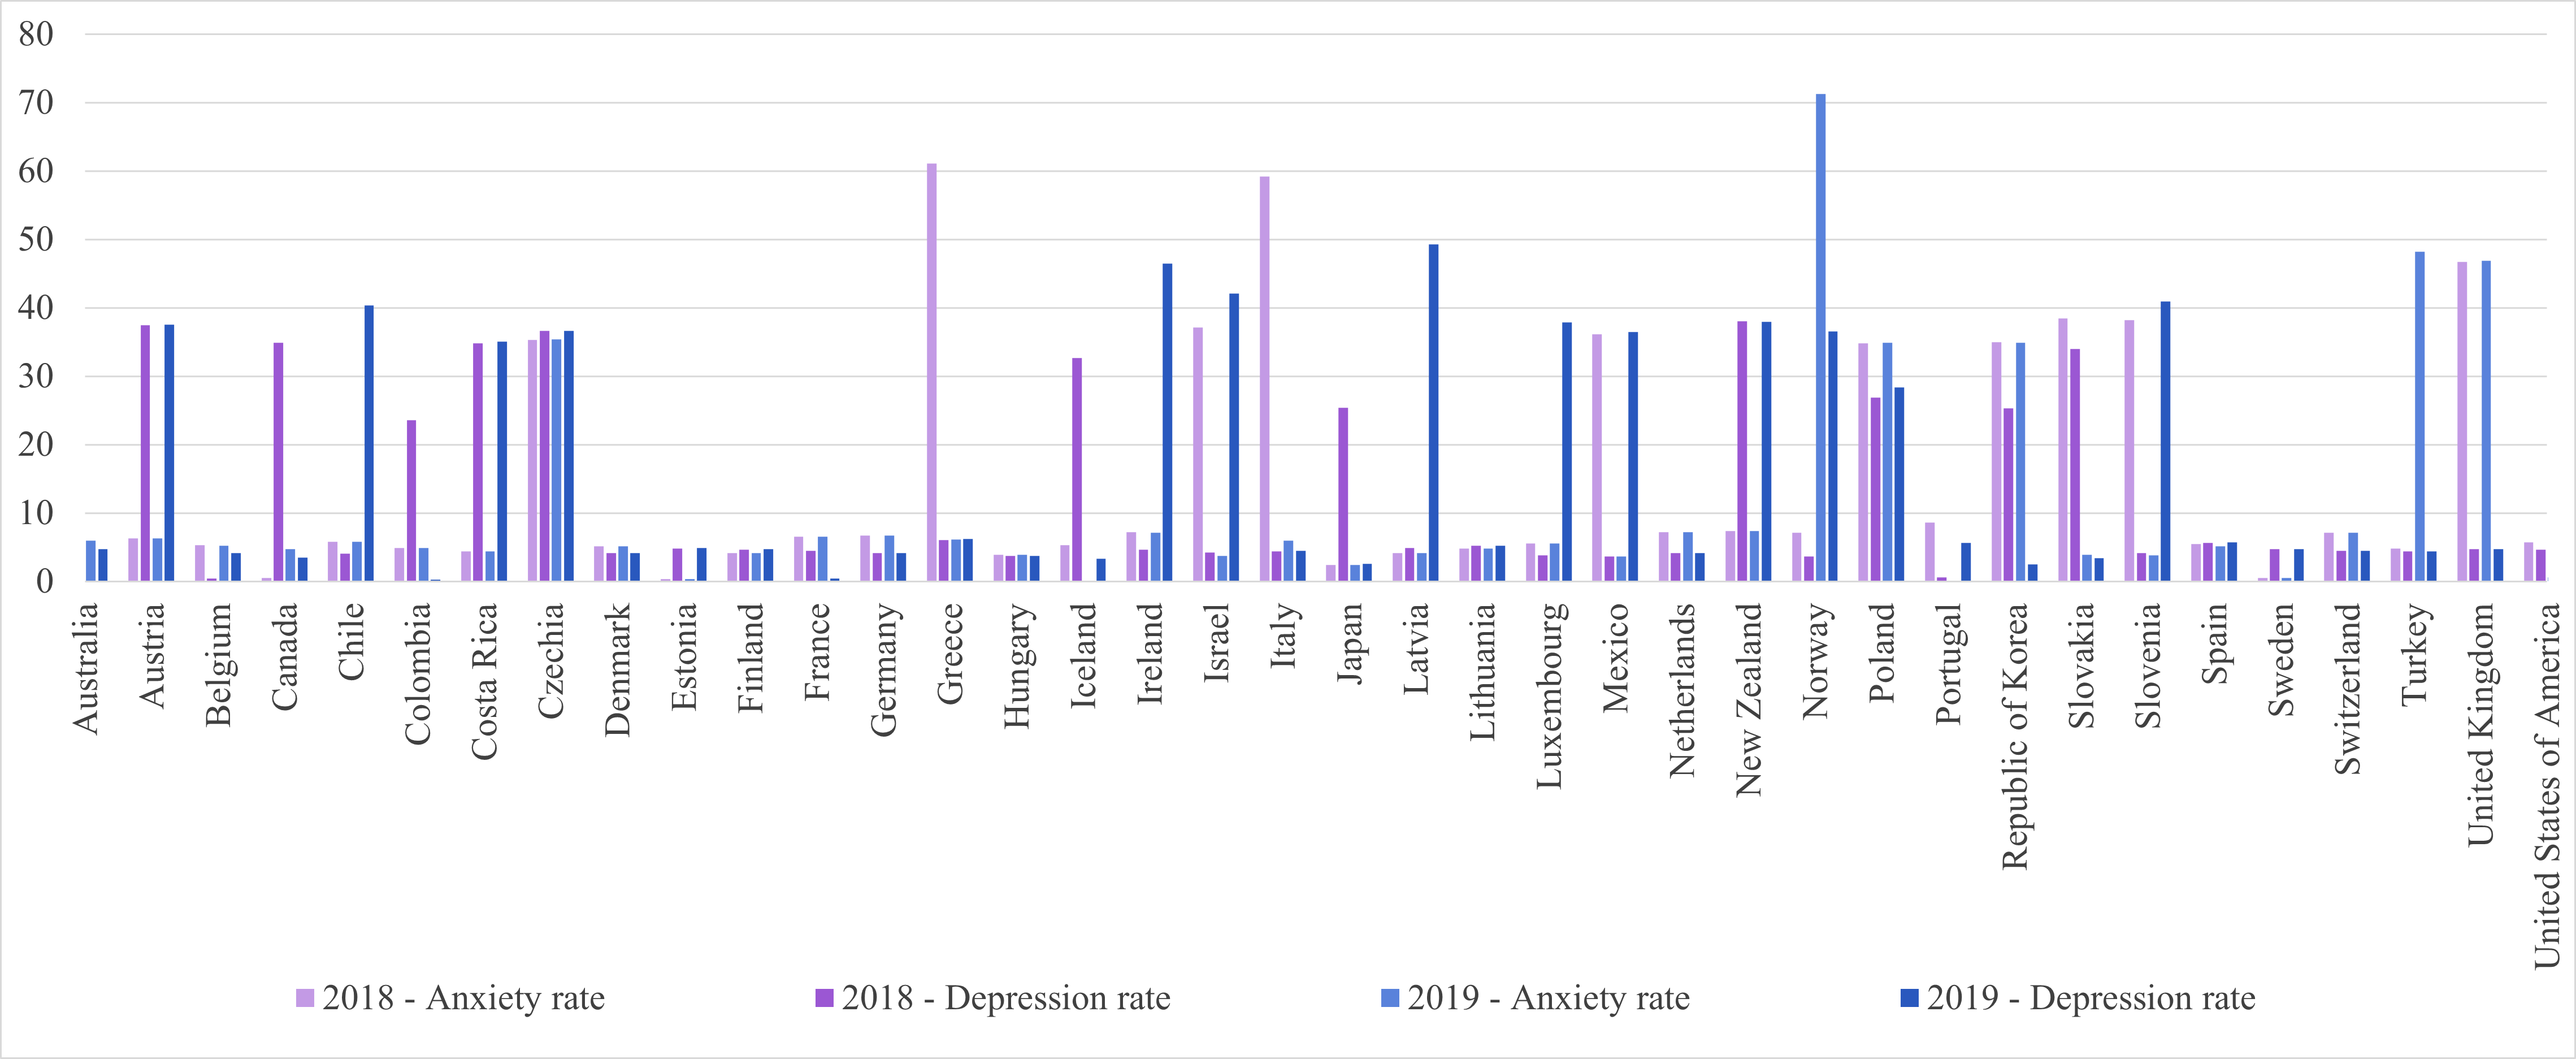
\includegraphics[width=\textwidth]{GRAPHS/anxiety_depression_100_rate_2018_2019.png}
                \caption{\emph{Prevalence of anxiety and depression disorders per $100$ inhabitants, 2018-2019.}
                {\scriptsize Source: Global Burden of Disease Study 2019 (GBD 2019), available from https://vizhub.healthdata.org/gbd-results/.}}
                \label{fig:anxiety_OECD}
            \end{figure}
            
            % DSM-V 
            Anxiety disorders involve excessive and prolonged feelings of worry, fear, or nervousness that negatively affect an individual's ability to function. According to the Fifth Edition of the Diagnostic and Statistical Manual of Mental Disorders (DSM-5), they are classified as follows: separation anxiety disorder, selective mutism, specific phobia (related to animals, natural environment, blood, injection, injuries, specific situations or other), social phobia, panic disorder, panic attacks, agoraphobia, generalized anxiety disorder (GAD). Comorbidity of anxiety disorders is most common with depression and substance abuse (DSM-5, WHO (2022)).

            The symptomatology includes physical symptoms that often include but are not limited to heart palpitations, muscle tension, and gastrointestinal discomfort. Behavioral symptoms manifest as avoidance behaviors, such as evading places or situations that trigger anxiety. On a psychological level, patients experience a heightened state of arousal and hyper-vigilance, frequently leading to intrusive thoughts and emotional distress. These symptoms are not static but interact in a dynamic fashion, often exacerbating each other in a vicious cycle that hampers the quality of life for the affected individual.


        % depression    [  %  TO DO  %  ]
        \subsection{Depressive disorders}
            According to the DSM-5 the main categories of depressive disorders are: major depressive disorder (MDD), persistent depressive disorder (dysthymia), bipolar depression, depressive disorder as a consequence of other medical conditions, and substance induced depressive disorder. For the disorder to be clinically relevant, the DSM-5 criteria must be met alongside functional impairment.
            Depressive disorders are often comorbid with anxiety disorders and substance abuse. 

            Core symptoms of this category include depressed mood, characterized by feelings of hopelessness, despair and sadness, and a significant loss of interest or pleasure in activities, also known as anhedonia. Depressive disorders are also characterized by the presence of cognitive symptoms such as reduced concentration, indecisiveness, feelings of worthlessness and guilt, and suicidal ideation. Additionally, symptoms may manifest physiologically through changes in appetite and weight, disturbed sleep, psychomotor issues in the form of agitation or retardation, and fatigue. Finally, an affected individual may show affective manifestations such as a lack of emotional responsiveness and irritability. 


    \subsection{Heterogeneity determinants of mental health conditions}
        Factors which generate heterogeneity in mental health measurement and statistics are gender, age, socio-economic status, ethnicity, geographic location, cultural background, sexual orientation. Furthermore, different diagnostic criteria and data collection methods complicate cross-country comparison. 
        For instance, cultural background adds a layer of complexity in the case of stronger stigma towards mental illness, which makes symptoms less readily identifiable and individuals more prone to masking their conditions.  
        To further exemplify the complexity from the interplay of the aforementioned factors, the reader may consider the fact that worldwide about 4\% of people live with anxiety disorders, but this number increases to 10\% for working age women in the Americas (WHO, 2022). 
        
        In this analysis, two of the most poignant determinants of heterogeneity are gender and cohort. 


    % statistics using WHO and EUROSTAT data references
    \paragraph{Gender differences.}
        % differences in diagnosis
        Women and men often display different prevalence rates and patterns of mental health issues.
        On average, women are more likely to be diagnosed with mood and anxiety disorders, such as depression and generalized anxiety disorder, while men are more prone to be diagnosed with substance abuse and externalizing disorders like conduct disorder (WHO, 2022). Worldwide, 13.5\% of women live with a mental disorder, as opposed to 12.5\% of men (WHO, 2022). 
        % pregnancy
        Factors such as pregnancy increase the risk of all mental conditions, especially depression. Woody et al. (2017) find increase prevalence of symptoms in women from low and middle income countries in the perinatal period. 
        % symptomatology of disorders
        Alexandrino-Silva et al. (2012) analyze symptomatics subtypes of depression and their relation to gender. For the most symptomatic classes of the disorders, they find women reporting more inhibition and disturbances to sleeping and eating patterns, and hypersomnia. Men reported more psychomotor retardation and agitation. 

    % MEN MORE LIKELY TO DIE SUCIDE    [   CHECK   ]

    \paragraph{Cohort specificity.}
    % youth and old more affected
    Youths and older adults suffer most from mental conditions. WHO (2022) data shows that around 8\% of children aged 5-9 and 14\% of adolescents ages 10-19 live with a mental condition. For adults 70 years and older, around 13\% live with a mental disorder (excluding dementia), mostly in the form of depressive and anxiety disorders. Within this age category, affected women are 14.2\% and men 11.7\%.

    % onset
    The analysis of a nationally representative survey in the United States done by Kessler et al. (2005) shows that the median age for onset is 11 years for anxiety disorders, 20 years for substance abuse and 30 years for mood disorders. Overall, three fourths of all lifetime conditions have onset before 24 years of age. 

    % old people problems: depression, anxiety, suicide, isolation      [   COMPLETE    ]
    In the older population, depression is associated with emotional suffering and increased suicidal ideation, and a risk factor for disability and mortality (Zenebe et al. (2021), Vieira et al., (2014)). Many of the risk factors for depression are associated with increased age, such as social isolation, traumatic life events, functional decline, loss of independence and onset of medical conditions. Depression in older adults is associated with events such as falls, strokes, functional ipairment, activity limitations (Vieira et al., 2014). A study on geriatric depression in the public community long-term care system by Morrow-Howell et al. (2008) found that 40\% of the sample was consistently depressed over a year of observations, with Comorbidity of medical, functional and psychosocial conditions.

    A similar picture can be drawn for anxiety disorders in older adults. A study by Schaub and Linden (2000) on the German population found a weighted overall prevalence of anxiety of 4.3\% for individuals aged 70-84 years old, higher than the 2.3\% observed in the group aged 85-103. Interestingly, this study also found no relation between anxiety and cognitive status or socio-economic status.

    In a particularly alarming trend, data from the World Health Organization (WHO) in 2022 indicate that individuals over the age of 70 experience a suicide rate more than double that of their younger counterparts.


 \section{COVID-19's mental burden}
    The COVID-19 pandemic has had a profound impact on mental health, manifesting in distinct but interconnected local and global threats. At the local level, individuals have reported higher rates of anxiety, depression and stress related symptoms, driven by exposure to risk factors such as social isolation, disruption to daily activities and heightened uncertainty. On a broader, structural scale, the pandemic has significantly compromised healthcare delivery, a disruption of particular impact for those with pre-existing mental health conditions (WHO, 2022). Overall, this has had a disproportionate impact on vulnerable and disadvantaged populations, further widening existing inequalities. 
    Public health emergencies of this kind can be platforms for change, driving improvement of public services and structural investments in the name of public interest, focused on education, prevention and effective treatment aimed at rehabilitation. 

    %   stressors
    The pandemic increased the prevalence and intensity of mental health stressors. The most palpable of these is fear of the health implications of the virus, a concern that was particularly acute during the periods of maximum uncertainty surrounding its nature and transmission. Contracting the virus introduces an additional layer of adversity, encompassing not just the physical symptoms, but also the psychological toll linked to the illness and its potential long-term effects. Additionally, the emotional burden of bereavement adds yet another dimension to the mental health landscape.
    Public health containment measures, such as distancing and quarantining, imposed social isolation and loneliness on many, generating feelings of helplessness and putting strain on the individual's relationships. Loss of routine and abrupt change to daily activities has negatively impacted the youth and the older component of the populations (WHO, 2022). 

    %   work
    COVID-19 exacerbated uncertainty for the work force, causing spikes in unemployment and plunging many into financial adversity. Both unemployment and poverty are known risk factors for mental health conditions, and gloabl projections for extreme poverty have been revised upwards in light of the pandemic (Lakner et al., 2020). 

    %   negative coping
    Negative coping mechanisms for psychological distress and symptoms of anxiety and depression may include resorting to alcohol, drugs and other addictive behavior, including but not limited to technology aided gambling, gaming and excessive use of social media. 



    
\chapter{Framing the Research Question}

Building upon the previous chapter's exploration of mental health, this chapter aims to frame the research question and provide a comprehensive and pertinent literature review. While there exists an extensive body of literature on mental health, both as an isolated subject and as a determinant of individual outcomes, much of this research is limited to correlational analyses. These studies often fall short of addressing the methodological challenges inherent in establishing a causal relationship between mental health conditions and individual outcomes.

Among the most commonly examined outcomes related to mental health are:
\begin{enumerate}
    \item \textbf{Labor Market Participation.} Including employment status, job performance, hours worked, wages, and self-rated satisfaction.
    \item \textbf{Physical Well-being.} Such as likelihood of hospitalization, quality of life, healthcare utilization, physical mobility, and dependence on external assistance.
    \item \textbf{Social Networks.} Measured by size and quality, self-reported satisfaction, frequency of social interaction, isolation, and perceived loneliness.
    \item \textbf{Community Involvement.} Including civic participation and elective activities.
\end{enumerate}

Additional outcomes may include behavioral ones such as the likelihood of substance use, financial stability, and educational ones like dropout rates, attainment, attendance, and performance.

Data collection for mental well-being is typically conducted using standardized questionnaires and scales, including Beck Depression Inventory (BDI), Generalized Anxiety Disorder 7 (GAD-7), Patient Health Questionnaire 9 (PHQ-9), Center for Epidemiological Studies-Depression Minus Loneliness (CES-D-ML), %  FINISH  % . 
These assessments are commonly administered via assisted face-to-face interviews or through computerized adaptive testing interviews (CATI). Observations made by the interviewer about the context and the respondent can be integrated to provide a more comprehensive understanding of the individual's state.

\section{Literature Review}
%   introduce the literature review
The existing literature on the topic is fragmented in both topics and methods, primarily due to challenges in sourcing appropriate data for investigation and different diagnostic tools employed to assess mental well-being in subjects. 
A frequently utilized dataset for this line of research is the Survey of Health, Ageing and Retirement in Europe (SHARE). This dataset provides a wealth of variables that are highly relevant to this study, thus the following literature review is particularly focused in its applications in researching mental health. Detailed information about SHARE, as well as other datasets employed in this dissertation, will be available in Chapter 3.


%   introduce the methodology for the literature review
    %   Clearly state what you aim to discover through this literature review
    %   Inclusion Criteria
    %   -   Peer-reviewed articles only.
    %   -   Published within a specific time frame (e.g., last 10 years).
    %   -   Articles must focus on empirical research.
    %   -   Articles must be available in English


\subsection{Mental Health and Labor Market Outcomes}
    The relationship between mental health and labor market outcomes is intricate, which may explain why existing research on the subject is limited and largely focuses on correlational findings. Labor market conditions encompass a wide range of factors, including job security, work-life balance, income levels, self-assessed job satisfaction, social support, and employment status. Additionally, specific working conditions—such as remote versus in-person work—and skill mismatches can influence an individual's mental well-being. In turn, these mental health states can also impact labor market outcomes. A systematic review by Rönnblad et al. (2019) investigated the effects of precarious employment on mental health, and mostly found very low quality evidence of negative effects of temporary employment or unpredictable work hours on mental health, and moderate quality of evidence was found for perceived job insecurity having adverse effects on mental health. 

    As an example of the many correlational studies, in Nadinloyi et al.'s (2013), the authors explore the correlation between job satisfaction and mental health among employees in two industrial firms. They assess individual conditions using Birfield's Job Satisfaction Scale and the Ruth Questionnaire and Scale. The study employs multiple regression analysis, t-tests, and Pearson correlation coefficients as its methodology. However, it does not address the potential issue of reverse causality between job satisfaction and mental well-being, thereby limiting the interpretation of the results to correlational rather than causal relationships. 

    In contrast to the method employed by Nadinloyi et al. (2013), Banerjee et al. (2017), Frijters et al. (2014) and Frijters et al. (2010) tackle endogeneity issues in two different ways. Banerjee et al. (2017) explore the impact of psychiatric disorders on labor market performance by utilizing a structural equation model that incorporates a latent index for mental health. This index is formulated based on symptoms from four specific psychiatric conditions (major depression, panic attacks, social phobia, and generalized anxiety disorder) as well as demographic, socioeconomic, and health-related variables. To address endogeneity, the study employs a Multiple Indicator and Multiple Cause (MIMIC) model, with the aid of covariance instruments. The findings reveal that mental illness negatively influences both employment rates and labor force participation. The study estimates that improving mental health could potentially increase employment for 3.5 million people and reduce absenteeism costs by approximately \$21.6 billion.
    Frijters et al. (2010) focus on the impact of mental health on employment status. Mental health is measured as an index based on the Short-Form General Health Survey (SF-36) answers. To tackle endogeneity concerns, their preferred specification is an Instrumental Variable (IV) Probit model, using the death of a close friends as an instrument for mental health to control for endogeneity concerns. The paper finds that a one standard deviation decline in mental health leads to a drop in the probability of labor market participation by around 19 percentage points. 
    Finally, Frijters et al. (2014) also measures mental well-being with the SF-36 Survey and exploits the death of a close friend as an instrument, however the method of choice is an Instrumental Variables Fixed Effects (IV-FE) model applied to high-quality Australian panel data spanning 10 waves. Results prove that mental health has a substantial negative impact on employment, with a one standard deviation in mental health leading to a 30 percentage point reduction in the likelihood of being employed. 


\subsection{Mental Health and Loneliness}
% difference between isolation and loneliness, and their relation
% relevance for mental health
    The body of literature exploring the relationship between loneliness and mental health faces the same methodological challenges, including issues of reverse causality, unobserved variables, and measurement errors in the independent variable. Studies in this domain can be categorized into three distinct groups: 
    1) pre-pandemic studies that largely fall short in adequately addressing endogeneity concerns; 
    2) research leveraging pandemic-related data to investigate the link between loneliness and mental health;
    3) a subset of papers employing more rigorous methodologies to provide credible insights into the relationship.

    Fokkema et al. (2012) employ a cross-country comparative approach to analyse loneliness among older adults. Health variables include perceived health, functional limitations, and problems with seeing or hearing, all measured on a 5-point scale ranging from 'excellent' to 'poor.' The study utilizes hierarchical logistic regression to explore the factors contributing to varying levels of loneliness across countries. The dependent variable, 'loneliness,' is assessed through a single-item measure derived from the CES-D (depression) scale.
    The findings indicate that countries with older populations, a higher proportion of women, and a greater number of unpartnered older adults tend to report elevated levels of loneliness. However, the unaddressed endogenous relationship between physical and mental health limits the causal interpretation of the results.

    A paper by Alves et al. (2014) aims at understanding the predictors of feelings of loneliness in middle-aged and older adults in Portugal through logistic regression analysis using survey data (socio-demographic variables, residence characteristics, measures of health). They find that variables such as age, gender, marital status, living arrangements, region, type of housing, professional status and income are all significantly associated with feelings of loneliness. 

    Niedzwiedz et al. (2016) investigates the relationship of loneliness and household wealth in older adults, focusing on the mediating role of social participation. Mental well-being is measured with the R-UCLA loneliness scale, and household wealth is measured by the sum of financial and real assets, minus liabilities. The authors recognize the limitations of a cross-sectional logistic regression study, and find that household wealth is associated with higher levels of loneliness. They also identify social participation as a key mediating factor, noting that certain forms of social engagement are particularly effective in alleviating loneliness.

    Logistic regression is also the tool of choice in Jarach et al. (2021), which uses SHARE data to investigate the relation between loneliness and the reversion of frailty in older Europeans. Loneliness is measured with the UCLA-L scale, and social isolation is measured with a custom index. 
    Multinomial logistic regression is used to compute relative risk ratios for changing frailty status according to levels of social isolation and loneliness. Their findings indicate that both loneliness and social isolation are significantly linked to the increased risk of individuals transitioning from a robust to a frail or pre-frail state.

    Loneliness may also have an association with cognitive impairment, as analysed by Luchetti et al. (2019), which investigate the relationship between loneliness and cognitive impairment using data from SHARE. To assess cognitive performance, they utilize the memory and verbal fluency tasks provided by SHARE, while employing the R-UCLA scale to gauge loneliness. The researchers opt for Cox regression hazard models to analyse the time-to-event relationship from baseline predictors to the onset of cognitive issues. Sensitivity analyses reinforce the robustness of their findings, revealing that loneliness is a significant predictor of cognitive impairment, even after adjusting for variables such as age, sex, education, and depressive symptoms.

    Lee et al. (2020) focus on exploring loneliness among older adults in the Czech Republic. They employ the UCLA-L scale to measure loneliness and use the EURO-D scale to evaluate mental and emotional health. While the study aims to understand the relationship between mental and physical health, its methodology is limited to regression analysis, analysis of variance (ANOVA), and descriptive statistics, without addressing the aforementioned endogeneity issues.

    Hajek and König (2022) employ SHARE longitudinal data and utilize linear fixed-effects regression to account for unobservable variables while investigating the factors associated with loneliness in older Europeans. Their analysis reveals that loneliness intensifies with factors such as aging, alterations in marital status, reductions in log income, deteriorating self-assessed health, and functional decline. Interestingly, they found no correlation between changes in chronic diseases and shifts in loneliness levels.

    In the second category of research papers on loneliness, the following studies were chosen for their use of pandemic-related data. Starting with a paper by Santini et al. (2021-A)
    The second study, by Atzendorf et al. (2022), examines the mental well-being of retired adults in various European countries during the COVID-19 pandemic, with a specific focus on loneliness and depression. The researchers utilized the SHARE Corona Survey, supplemented by the Oxford Government Response Tracker (OxGRT), to gather data on individual feelings of loneliness and depression with respect to pre-pandemic times, and on the stringency of epidemic control measures. Their methodological approach involved multilevel binary logistic regression models that incorporated both individual and country-level variables. The authors find significant differences between countries in the prevalence of increased feelings of depression and loneliness, particularly for the oldest in the sample. Specifically, the number of deaths explains 32.4\% of the country variance in depression and 20.7\% in loneliness.
    The third study, conducted by Arpino et al. (2022), assesses the effects of the COVID-19 pandemic on loneliness in older adults. It specifically explores how variables such as childlessness and lack of a partner contribute to feelings of loneliness. The researchers chose to use the most recent wave of the SHARE dataset for their analysis. Employing a logistic model, they focused on the binary outcome variable of 'loneliness.' Their findings reveal that 11.6\% of respondents felt lonelier during the pandemic, while the overall prevalence of depression rose by 0.8\%. Being childless or unpartnered was a significant risk factor for increased feelings of loneliness. 

    Finally, a paper by Santini et al. (2020) stood out by addressing endogeneity in the analysis of the relationship between social disconnectedness, perceived isolation, and symptoms of depression and anxiety in older adults using longitudinal data from the National Social Life, Health, and Aging Project (NSHAP) in the USA. 
    The method of choice is a random intercept cross-lag panel model with maximum likelihood estimation. According to the authors, this approach aims to establish whether the associations might have been obtained spuriously based on stable third variable traits that were not controlled for. The authors also acknowledge the potential for measurement error, noting that results could vary if mental health were assessed through clinical evaluations rather than screening tools. Additionally, they recognize unaccounted-for confounders like stressful life events or a family history of mental disorders. 
    Their findings indicate that social disconnectedness leads to perceived isolation, which subsequently predicts depression and anxiety. To address concerns of reverse causality, the authors also explored the reverse relationships between variables and found evidence supporting bi-directional influences.


\subsection{Mental Health and Social Capital}
    Mental health and social capital are linked by a mutually reinforcing relationship, creating a cycle that affects both individual and collective well-being. Poor mental health can hinder an individual's ability to accumulate social capital by reducing productivity and limiting social engagement. Conversely, a lack of social capital can exacerbate mental health issues due to diminished social support, community cohesion, and access to quality information. Additionally, societal stigma and economic disadvantages associated with low social capital further impact mental well-being.

    %   sirven debrand  2012
    In their 2012 study, Sirven and Debrand employ panel data from the SHARE and SHARELIFE surveys to explore the causal relationships between social capital and health in an older European population. The authors employ a comprehensive set of baseline health indicators, encompassing both physical dimensions (such as poor self-rated health, limitations in Activities of Daily Living (ADL), General Activity Limitations Indicator (GALI), mobility restrictions, and low grip strength) and mental aspects (such as depressive symptoms and cognitive impairment). Given the bidirectional causality between mental health and overall well-being, addressing endogeneity is crucial for establishing the causal implications of their findings. While acknowledging the merits of an Instrumental Variables (IV) approach, the authors express reservations about its ability to accurately assess the impact of social capital on health when using various social capital measures. Instead, they opt for a bivariate recursive probit model, incorporating lagged values of the dependent variables to account for endogeneity.
    The results suggest a reciprocal causal relationship between social capital and health. Specifically, past health statust influences individual health in the following period, and the same relationship holds for social participation. The impact of health on social capital is found to be more substantial than the reverse, indicating that health may serve as a more potent driver for the accumulation or depletion of social capital. 

    %   murayama        2013
    Murayama et al. (2013) investigates the longitudinal effects of bonding and bridging social capital on self-rated health, depressive mood, and cognitive decline among older Japanese individuals. Utilizing panel data from the Hatoyama Cohort Study, the research focuses on social capital as the key independent variable, where bonding social capital is assessed based on the individual's perception of neighborhood and network homogeneity, while bridging social capital is assessed based on the individual's perception of network heterogeneity.
    The study finds that stronger perceived neighborhood homogeneity is inversely associated with poor self-rated health and depressive mood. However, neither bonding nor bridging social capital was significantly associated with cognitive decline.
    The authors employ logistic regression models to carry out their analysis, however, they do not explicitly address the critical issue of endogeneity, particularly the problem of reverse causality between social capital and health outcomes. 

    %   eshan de silva  2015
    Ehsan and De Silva (2015) present a systematic review that investigates the association between social capital and common mental disorders, such as depression, anxiety, and PTSD, using validated measurement tools. While the review includes a large number of studies, it does not directly tackle the issue of endogeneity in the methodologies of the reviewed works. Additionally, the authors note that the majority of the studies are situated in middle to high-income countries, limiting the generalizability of the findings to lower-income settings.

    %   riumallo        2014
    A paper focused on yet another high-income country is Riumallo et al. (2014), which explores the relation between social capital and both self-rated health and biological health in Chile using data from the Chilean National Health Survey (2009-2010). Using an IV approach with a variety of instruments, they define the dependent variable using a binary indicaotr of self-rated health, depression, hypertension or diabetes. Social capital is captured by a questionnaire inquiring about social support, generalized trust and neighborhood trust. The study uses recent crime victimization and aggregate social capital as instruments, and finds that all social capital indicators have an association with depression. Some social capital indicators are associated with self-rated health, hypertension and diabetes above age 45.

    %   landestedt      2016
    A paper by Landstedt et al. (2016) focuses on the longitudinal relationship between individual-level structural social capital, measured as civic engagement, and depressive symptoms from age 16 to 42 in Swedish men and women, using data from the Northern Swedish Cohort. Civic engagement is measured by a single-item question reflecting the level of engagement in clubs or organizations, and depressive symptoms are measured with an index.
    Methodologically, the authors employ cross-lagged structural equation models separated by gender in order to analyze the directions of associations between civic engagement and depressive symptoms. The directionality between social capital and mental health is established with the use of a cross-lagged structural equation model, which explains present values of the dependent with past values of the independent variable. Results show that both civic engagement and depressive symptoms are stable across time, with male civic engagement being inversely related to depressive symptoms in adulthood, while no such relationship is observed for women. 

    %   cohen cline     2018
    Finally, a paper by Cohen-Cline et al. (2018) explores the relationship between social capital and depression, utilizing a sample of same-sex twin pairs. Symptoms of depression are measured with the Patient Health Questionnaire (PHQ-2); social capital is conceptualized into cognitive and structural domains, with the former including sense of belonging, neighborhood social cohesion, trust and workplace connections, and the latter is measured through volunteerism, community participation, and social interaction.
    The twin design combined with a Poisson model offer an approach that controls for genetic and environmental confounders. However, this does not necessarily translate to solving the ever-present issue of reverse causality. 
    Results show that all measures of cognitive social capital and neighborhood characteristics are associated with less depressive symptoms. 
    

\subsection{Mental Health and Social Networks}
    The topic of social capital is tightly linked with the nature of social networks since their quality serves as a critical dimension of social capital, shaping its effectiveness and impact on mental well-being. High-quality networks, characterized by strong, trust-based relationships, not only facilitate the exchange of valuable information but also provide emotional support and a sense of belonging. These factors contribute to a more robust form of social capital, which in turn positively influences mental health by building resilience and fostering self-esteem (WHO, 2022). Conversely, low-quality social networks, marked by weak ties and low levels of trust, can diminish social capital and exacerbate mental health issues. Therefore, the quality of one's social network is a pivotal factor in the symbiotic relationship between social capital and mental health.
    An individual's social network can be characterized by three key dimensions: the quantity of connections, the quality of those connections, and the geographical proximity to other network members. 
        

    %   shiovitz    2010
    Shiovitz-Ezra and Leitsch (2010) explores the associations between objective and subjective social network characteristics and their impact on loneliness in older adults. Mental health is measured with the R-UCLA scale, and subjective measures such as eyesight and hearing loss. The paper distinguishes between objective indicators like frequency of contact with social network members and subjective perceptions of social ties, such as the quality of marriage or familial relationships. Results show that a larger portion of the variance in loneliness perception is explained in the non-married sub-sample, 13\%, relative to the married or cohabiting sub-sample, 7\%.
    The empirical strategy of the paper involves the use of hierarchical linear regression models applied to a cross-section of the NSHAP dataset. This specification does not properly account for reverse causality:  individuals who are lonely or have mental health issues might have fewer social interactions or perceive their social networks differently. In addition, the model does not adequately address likely omitted variable bias and simultaneity.

    %   gu          2020
    Another correlative paper is found in Gu (2020), which aims to explore the impact of neighborhood social networks on the mental well-being of women residents in a middle-class urban neighborhood in Seoul, South Korea. The study employs a phenomenological qualitative approach, an approach that translates to dialogical interviews to understand the pehonmenon, and focuses on 18 full-time or part-time housewives with children. Results are ambiguous and highly context specific, showing both positive and negative effects on the women's well-being.

    %   santini     2021-B
    Santini et al. (2021-B) investigates the moderating role of social network size in the relationship between formal social participation and mental health outcomes among older adults in Europe, focusing specifically on quality of life and symptoms of depression. The dataset of choice is SHARE (waves from 2011 and 2013) to investigate formal social participation and social network size, with their impact on quality of life and depressive symptoms. The moderating role of formal social participation is investigated through a linear regression model with two possible outcomes: quality of life, as measured by the CASP-12 scale, and depressive symptoms, measured with the EURO-D scale. Although results show that individuals with few social ties may benefit from social participation via a reduction in depressive symptoms and an increase in quality of life, the specification choices raise concerns analogous to those discussed for Shiovitz-Ezra and Leitsch (2010).

    %   coleman     2022
    Finally, Coleman et al. (2022) examine how social networks prior to the pandemic influenced older adults in perceived risk of COVID-19, preventative behavior and mental health outcomes such as loneliness, depression and enxiety. The authors distinguish between bridging and bonding social capital. Specifically, bridging social capital refers to the benefits derived from a vast and diverse social network, while bonding social capital refers to the benefits derived from strong and close ties in a social network. The former manifests in weak ties, and is found to predict a higher perceived risk of COVID-19, as well as more preventative behaviors; the latter is associated with less perceived COVID-19 risk, fewer precaution, but better mental health outcomes. The authord fit 60 models using ordinary least squares (OLS) regression for for continuous outcome variables (risk perception, loneliness, stress), binomial regression for count outcomes (health precautions, depression, anxiety), and generalized linear models (GLM). To accredit causal interpretation of the results, controls for baseline mental health are included in the model. According to the authors, the use of a cross-lagged approach and the timing of data collection should mitigate concerns of reverse causation.
    Results show that mean density of the network, mean tie strength and strength of the weakest tie are significantly associated with loneliness. For depressive symptoms, lower values are associated with mean support functions received from the network, mean tie strength, and strength of the weakest tie. Finally, proportion of frequent contact, diversity, and strength of weakest tie are associated with lower anxiety, while network density is associated with higher anxiety, therefore suggesting that bonding capital can be negatively associated with mental health. 



\section{Summary and Implications}
In this literature review I aimed to provide a comprehensive examination of the existing research on the interplay of mental well-being and various outcomes such as labor market participation, loneliness, and social capital (with additional focus on social networks). I have highlighted the methodological challenges in establishing a causal relationship between mental health and outcomes, particularly the issues of reverse causality and simultaneity. While some studies address these challenges with various methods, many fall short, proving the need for rigorous approaches in this field. By underlining the shortcomings of the literature in question, I have set the stage for the empirical analysis in the following chapters, with the aim of contributing to filling the gaps about the evidence of a causal link. 




    \chapter{data}

% describe variables already in dataset AND created vars

% SHARE 

% OxGRT

    \chapter{strategy}
    \chapter{estimation}
    \chapter{discussion}
    \chapter{conclusion}
    \chapter{references}
    \chapter{appendix}




\backmatter




\end{document}